\chapter{Ensemble microcanonico}
Il concetto fondamentale alla base dell'approccio statistico consiste, per un'osservabile $O$, nella relazione
\begin{equation}
    O = \nsum_\nu P(\nu)O(\nu) \equiv \vmedio{O},
\end{equation}
dove $\{\nu\}$ è l'insieme dei microstati compatibili con lo stato macroscopico del sistema considerato e $\vmedio{O}$ è una media statistica sull'insieme di tali microstati, in quanto pesata con la probabilità $P(\nu)$. Per poter sfruttare questo approccio è necessario:
\begin{enumerate}
    \item determinare la forma generale di $P(\nu)$ per i diversi tipi di sistemi in funzione delle variabili microscopiche;
    \item esprimere le quantità termodinamiche rilevanti per i diversi sistemi in termini di $P(\nu)$.
\end{enumerate}
L'ensemble microcanonico corrisponde ad un sistema isolato:
\begin{enumerate}
    \item chimicamente, quindi il numero di particelle $N$ è fissato e non avvengono decadimenti e/o aggregazioni;
    \item meccanicamente, per cui il volume $V$ è finito e il sistema non si espande e comprime;
    \item termicamente, ovvero le pareti del contenitore non permettono uno scambio di energia $E$.
\end{enumerate} 
Pertanto, le variabili di controllo consistono in $\{E,V,N\}$, tutte grandezze di carattere estensivo. Quindi, l'ensemble microcanonico è l'ensemble dei microstati che il sistema può assumere quando sono fissate queste variabili. Tuttavia, nella realtà non si può fissare completamente l'energia, infatti si ha un'inevitabile incertezza per cui i microstati $\nu$ dell'ensemble microcanonico con energia $E$ sono tali che
\begin{equation}
    E \le E(\nu) \le E + \Delta,\quad \frac{\Delta}{E} \ll 1.
\end{equation}
Se ci si pone nello spazio delle fasi, si osserva che i microstati si trovano su un livello di energia definita dall'ipersuperficie di energia fissata $E$ e dalla corona $E + \Delta$, come mostrato in figura \ref{fig: spazio delle fasi microcanonico}.
\begin{figure}[h]
    \centering
    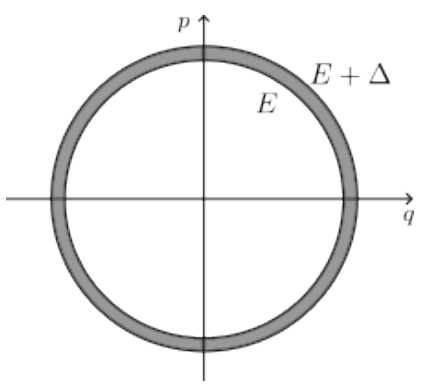
\includegraphics[width=0.35\linewidth]{Immagini/spazio delle fasi microcanonico.png}
    \caption{ensemble microcanonico dei microstati nello spazio delle fasi.}
    \label{fig: spazio delle fasi microcanonico}
\end{figure}

All'equilibrio, si può assumere che la probabilità $P(\nu)$ dipenda solo dall'energia, in quanto, dato che deve essere stazionaria, deve avere parentesi di Poisson nulle con l'operatore di Liouville nel caso classico, dove $P(\nu) \equiv \rho(q,p)$, o con l'hamiltoniana nel caso quantistico, potendo quindi dipendere solo da costanti del moto, in questo caso l'energia $E$. Essendo l'energia $E$ fissata per tutti i microstati, anche $P(\nu)$ deve esserlo, ma allora è anche indipendente da $\nu$ e tutti i microstati sono equiprobabili. Sia ora $\Omega(E,V,N)$ il numero di $\nu$ nell'ensemble, ossia il numero di quelli che si trovano nello stesso livello di energia, allora la condizione di normalizzazione della probabilità $P(\nu) \equiv P$ implica che 
\begin{equation}
\label{eq: probabilità microstati (microcanonico)}
    \sum_{\nu = 1}^\Omega P(\nu) = \Omega P = 1\quad\Rightarrow\quad P = \frac{1}{\Omega(E,V,N)}.
\end{equation}

\subsubsection{Ergodicità}
In generale, un sistema isolato è descrivibile tramite l'ensemble microcanonico se la media temporale delle osservabili è effettivamente uguale alla media di ensemble 
\begin{equation}
\label{eq: media ensemble microcanonico}
    \bar{O} = \sum_{\nu = 1}^\Omega P(\nu)O(\nu) = \frac{1}{\Omega}\sum_{\nu = 1}^\Omega O(\nu),
\end{equation}
cioè se, per tempi sufficientemente lunghi, il sistema visita tutti gli stati accessibili con la stessa frequenza. Un sistema che presenta tale comportamento è detto ``ergodico''. Nel suo moto sul livello di energia fissata, il sistema passa arbitrariamente vicino ad ogni punto, ossia ad ogni microstato, ed il tempo che trascorre in ognuna sottoregione è proporzionale all'area della stessa. 

Tuttavia, l'ergodicità di un sistema dinamico a molti corpi è difficile da stabilire rigorosamente, anche se i sistemi reali, in buona approssimazione, sono quasi sempre ergodici. Si presentano infatti alcuni problemi:
\begin{enumerate}
    \item secondo il teorema KAM anche sotto perturbazioni, certi sistemi dinamici continuano a seguire traiettorie confinate in certe sottoregioni individuate dalle condizioni iniziali, non diventando mai caotici;
    \item nelle simulazioni numeriche il comportamento ergodico fatica ad emergere.
\end{enumerate}
Anche ammettendo che ci fosse un comportamento ergodico, la media statistica \eqref{eq: media ensemble microcanonico} sarebbe giustificata se il tempo di misura $t$ fosse comparabile con il tempo di ritorno $T$ impiegato dal sistema per ritornare nei pressi dello stato iniziale. Tuttavia, se nella dinamica c'è una piccola componente causale, necessaria per la termalizzazione, allora per il lemma di Kac ci si può aspettare che il tempo di ritorno cresca esponenzialmente con il numero di componenti, e quindi i tempi di ritorno siano estremamente lunghi 
\begin{equation}
    T \simeq \tau_c e^{\alpha N},
\end{equation}
dove $\tau_c$ è il tempo di scala della collisioni molecolari e $\alpha$ è lo stesso coefficiente che compare per la probabilità di un microstato, la quale invece decresce in funzione di $N$ come $P(\nu) \simeq e^{-\alpha N}$. Dunque, il tempo di ritorno $T$ è in genere fuori scala per qualsiasi applicazione reale, pertanto l'ergodicità potrebbe nella pratica essere una condizione irrilevante. 

D'altra parte, le osservabili di interesse in Termodinamica sono tipicamente one-body o two-body, quindi ciò che ci interessa realmente è che per tali osservabili valga l'uguaglianza \eqref{eq: media ensemble microcanonico} per quasi tutte le condizioni iniziali e sia approssimativamente valida nel limite $N\to\infty$ anche per tempi $t$ relativamente brevi e non
comparabili con il tempo di ritorno. Esistono risultati rigorosi nel contesto dei gas ideali e/o con interazioni a corto raggio che mostrano che tali osservabili sono in effetti ``self-averaging'': per $N\to\infty$ assumono un valore praticamente costante su quasi tutti i microstati accessibili e pertanto la media temporale viene a coincidere con la media statistica. 

\section{Entropia microcanonica}
Determinata la distribuzione di equilibrio, l'obiettivo adesso è quello di determinare la termodinamica, in particolare trovando un'espressione dell'entropia. Ci si aspetta che $\Omega(E,V,N)$ sia legato alla funzione che determina la termodinamica a fissate $\{E,V,N\}$, ovvero all'entropia $S(E,V,N)$. Si deve pertanto dedurre la relazione tra $\Omega$ e $S$. Per farlo, si considerano due sistemi microcanonici all'equilibrio termico posti a contatto, come mostrato in figura \ref{fig: sistemi per entropia (microcanonico)}. I due sistemi sono inizialmente isolati da una barriera, per cui il numero complessivo di microstati è
\begin{equation}
    \Omega(E) = \Omega_1(E_1,V_1,N_1)\Omega_2(E_2,V_2,N_2) \equiv \Omega_1(E_1)\Omega_2(E_2),
\end{equation}
data l'indipendenza dei due sistemi e l'invarianza dei due volumi e dei numeri di particelle in ciascuno di essi. 
\begin{figure}[h]
    \centering
    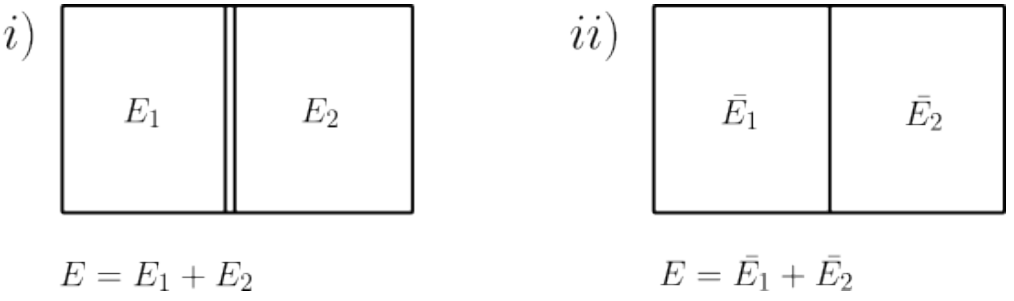
\includegraphics[width=0.65\linewidth]{Immagini/sistemi per entropia (microcanonico).png}
    \caption{sistemi nello stato: (i) iniziale e separati; (ii) finale e uniti.}
    \label{fig: sistemi per entropia (microcanonico)}
\end{figure}
Quando la barriera viene rimossa, i due sistemi sono posti a contatto e avviene uno scambio termico, pur rimanendo il sistema globalmente isolato. In questo momento il sistema non è più in equilibrio e nuovi microstati diventano disponibili con una diversa distribuzione di energia tra i due sottosistemi. Quindi, il numero di microstati possibili ora è dato da
\begin{equation}
\label{eq: microstati complessivi (microcanonico)}
    \Omega(E) = \int dE_1\,\Omega_1(E_1)\Omega_2(E_2),\quad E_2 \equiv E - E_1.
\end{equation}
L'idea consiste nel pensare che $\Omega(E)$ tende a evolvere fino a raggiungere un valore massimo nella nuova situazione di equilibrio, per un certo valore $\bar{E}_1$ e $\bar{E}_2 = E - \bar{E}_1$ delle energie dei due sistemi. Infatti, all'equilibrio, tra tutti i possibili valori di $E_1$ c'è uno che domina, contrassegnato da $\bar{E}_1$. Dunque, si assume che il macrostato di equilibrio sia quello che corrisponde al maggior numero possibile di microstati. 

Per vedere ciò, si considera un sistema composto da un gas inizialmente preparato in una situazione fuori equilibrio. Le componenti sono confinate in una sottoregione delimitata da una barriera, ma alla rimozione di questa il gas tende ad espandersi arrivando all'equilibrio occupando tutto il volume disponibile, come mostrato in figura \ref{fig: evoluzione sistema (microcanonico)}. 
\begin{figure}[h]
    \centering
    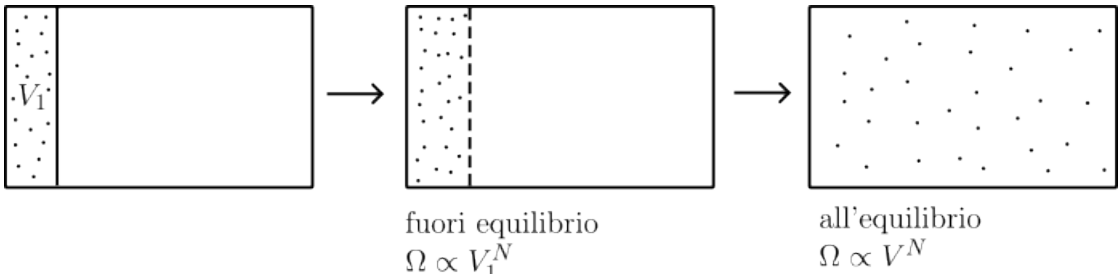
\includegraphics[width=0.75\linewidth]{Immagini/evoluzione sistema (microcanonico).png}
    \caption{evoluzione temporale di un gas verso lo stato di equilibrio.}
    \label{fig: evoluzione sistema (microcanonico)}
\end{figure}
A livello classico, il numero di microstati disponibili è proporzionale al volume dello spazio delle fasi permesso, in particolare cresce con il volume $V$ secondo $V^N$. Appena viene rimossa la barriera $\Omega \propto V_1^N$, ma avvicinandosi all'equilibrio, il sistema tende a massimizzare i microstati disponibili passando a $\Omega \propto V^N \gg V_1^N$. L'assunzione che $\Omega$ cresca all'avvicinarsi dell'equilibrio suggerisce già che questo sia collegata all'entropia. Tornando all'espressione \eqref{eq: microstati complessivi (microcanonico)}, nel limite termodinamico $\Omega_1$ tende ad essere molto piccata intorno ad $\bar{E}_1$, per cui l'integrale sarà dominato dalla zona nei pressi di $\bar{E}_1$ ed $\Omega(E)$ sarà massimo quando l'integrando in tale regione è massimo. 
\begin{notz}
    Per semplicità, nel seguito si pone $\bar{E}_1 \equiv E_1$.
\end{notz}
Pertanto, per massimizzare $\Omega(E)$ è sufficiente massimizzare l'integrando ottenendo
\begin{equation}
    \frac{\p}{\p E_1}[\Omega_1(E_1)\Omega_2(E_2)] = 0\quad\Rightarrow\quad \frac{\p\Omega_1}{\p E_1}\Omega_2(E_2) = \Omega_1(E_1)\frac{\p \Omega_2}{\p E_2}\bigg|_{E_2 = E - E_1},
\end{equation}
da cui si ricava la condizione di equilibrio 
\begin{equation}
\label{eq: condizione equilibrio (microcanonico)}
    \frac{\p\log{\Omega_1}}{\p E_1} = \frac{\p\log{\Omega_2}}{\p E_2}.
\end{equation}
Inoltre, dalla Termodinamica è noto che due sistemi sono in equilibrio se e solo se hanno la medesima temperatura, per cui all'equilibrio, sfruttando l'equazione di stato termica, si deve avere
\begin{equation}
\label{eq: condizione equilibro (TD)}
    \frac{1}{T_1} = \frac{\p S}{\p E_1}\bigg|_{V_1,N_1} = \frac{\p S}{\p E_2}\bigg|_{V_2,N_2} = \frac{1}{T_2}.
\end{equation}
Dunque, confrontando le relazioni \eqref{eq: condizione equilibrio (microcanonico)} e \eqref{eq: condizione equilibro (TD)} risulta naturale proporre come forma dell'entropia 
\begin{equation}
\label{eq: entropia (microcanonico)}
    S(E,V,N) = k\log{\Omega(E,V,N)}.
\end{equation}
Dall'espressione \eqref{eq: entropia (microcanonico)} si nota che l'entropia è una funzione della variabili estensive di controllo e che si avrebbe potuto aggiungere una costante additiva nella formula dell'entropia, consistita dal confronto delle relazioni \eqref{eq: condizione equilibrio (microcanonico)} e \eqref{eq: condizione equilibro (TD)}, ma non si è introdotta per rispettare il terzo principio della Termodinamica, il quale afferma che $S = 0$ se $\Omega = 1$, ossia quando è disponibile un unico microstato\footnote{In realtà non è sempre vero in quanto si potrebbe avere una degenerazione per cui $\Omega > 1$ anche per $T\to0$.}. Quest'ultimo caso corrisponde a ciò che accade allo zero assoluto, in cui il sistema può occupare unicamente lo stato fondamentale. 

Inoltre, considerando l'unione di due sistemi $\Omega_{12} = \Omega_1\Omega_2$, dalla \eqref{eq: entropia (microcanonico)} segue che $S$ è una quantità additiva, per cui $S = S_1 + S_2$, rispettando così l'estensività. Fatto ciò, nel seguito si considerano alcuni semplici ed importanti esempi di come estrarre la termodinamica tramite l'ensemble microcanonico, sia nel contesto classico con quello quantistico. 

\subsubsection{Sistemi quantistici}
Nell'ensemble microcanonico tutti i microstati sono equiprobabili, per cui data una base di stati stazionari $\{\ket{n}\}$, con $n = 1,\dots,\Omega$, a cui sono associate le energie $E_n \in [E,E + \Delta]$, la matrice densità $\rho_{mn}$ deve restituire l'informazione che gli stati sono equiprobabili. Per vederlo, si ricorda che $\hatrho$ è diagonale e, in base alla \eqref{eq: matrice densità diagonale}, quindi nella base degli autostati dell'energia si ha 
\begin{equation}
    \hatrho_{mn} = \frac{\delta_{mn}}{\Omega}.
\end{equation}
Pertanto, l'operatore $\hatrho$ si può scrivere come
\begin{equation}
    \hatrho = \frac{1}{\Omega}\nsum_n\ket{n}\bra{n} = \Omega^{-1}\MI,
\end{equation}
per cui i suoi autovalori sono tutti uguali e valgono $\lambda_n = \Omega^{-1}$. Ricordando la definizione dell'entropia di von Neumann \eqref{eq: definizione entropia von Neumann} per uno stato misto e dato che la traccia di $\hatrho$, essendo diagonale, è invariante rispetto alla scelta della base, ci si può porre in quella degli autostati dell'energia ottenendo
\begin{equation}
    \SvN = -\nsum_n\lambda_n\log{\lambda_n} = \log{\Omega}.
\end{equation}
Ora, se si postula che l'entropia $S$ sia data da $S = k\SvN$, allora si ottiene proprio l'entropia microcanonica \eqref{eq: entropia (microcanonico)}. Siccome $\hatrho \propto \MI$, mantiene la medesima espressione in ogni base, in una generica $\{\ket{\alpha}\}$ si ha ancora
\begin{equation}
\label{eq: operatore e matrice densità in una base generica (microcanonico)}
    \hatrho = \frac{1}{\Omega}\nsum_\alpha\ket{\alpha}\bra{\alpha},\quad\rho_{\alpha\beta} = \frac{\delta_{\alpha\beta}}{\Omega}.
\end{equation}
Tuttavia, in tale base non è detto che a priori $\hatrho$ all'equilibrio sia diagonale, in quanto $\hatrho$ deve commutare con $\hatH$, ma quest'ultima a sua volta non è diagonale. Per postulare l'espressione microcanonica \eqref{eq: operatore e matrice densità in una base generica (microcanonico)} in una base qualsiasi si fa uso di due assunzioni aggiuntive:
\begin{enumerate}
    \item l'equiprobabilità dei microstati, che conduce ai termini $\Omega^{-1}$ sulla diagonale;
    \item il postulato delle fasi causali, che afferma che l'ensemble microcanonico è una sovrapposizione incoerente di stati stazionari e che richiede anche l'annullamento dei termini non diagonali di $\rho_{\alpha\beta}$.
\end{enumerate}

\section{Gas ideale nell'ensemble microcanonico}
Si consideri un sistema composto da un gas di $N$ particelle identiche, di massa $m$ e non interagenti. Anche se le interazioni, pur trascurabili essendo a corto raggio, sono necessarie per la termalizzazione del sistema, si assume che l'hamiltoniana sia semplicemente
\begin{equation}
    H(q,p) = \frac{1}{2m}\sum_{i=1}^N|\vp_i|^2 \equiv \frac{1}{2m}\sum_{I=1}^{3N}|p_I|^2.
\end{equation}
L'ensemble microcanonico corrisponde alla sottoregione dello spazio delle fasi $\R^{6N}$ in cui l'hamiltoniana soddisfa la relazione
\begin{equation}
\label{eq: vincolo hamiltoniana gas ideale (microcanonico)}
    E \le H(q,p) \le E + \Delta,\quad \Delta \ll E.
\end{equation}
Pertanto, non è presente alcun vincolo sulle coordinate spaziali, a parte la condizione di essere all'interno del volume finito $V$. Mentre la condizione sull'hamiltoniana \eqref{eq: vincolo hamiltoniana gas ideale (microcanonico)} nello spazio delle fasi individua una sottoregione corrispondente ad una corona circolare di spessore $\Delta$ intorno ad un'ipersfera $(3N - 1)$-dimensionale di equazione
\begin{equation}
    \nsum_I|\vp_I|^2 = 2mE \equiv R^2(E),\quad R(E) := \sqrt{2mE}.
\end{equation}
Il volume di questo livello di energia, sviluppando secondo Taylor essendo $\Delta \ll E$, è
\begin{equation}
    \vps_p \simeq A_{3N-1}[R(E)][R(E + \Delta) - R(E)] \simeq \hatA_{3N - 1}R(E)^{3N - 1}\frac{\p R}{\p E}\Delta,
\end{equation}
dove $A_{3N-1}$ è l'area dell'ipersfera $S^{3N-1} \subset \R^{3N}$ di raggio $R$, raffigurata in figura \ref{fig: spazio delle fasi microcanonico (gas ideale)}. 
\begin{figure}[h]
    \centering
    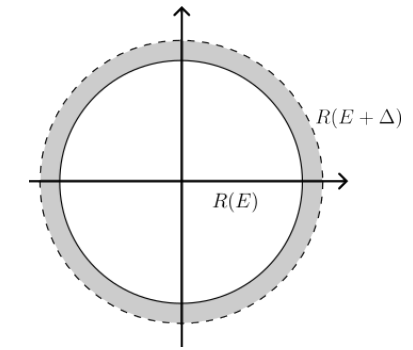
\includegraphics[width=0.4\linewidth]{Immagini/spazio delle fasi microcanonico (gas ideale).png}
    \caption{ensemble microcanonico di un gas ideale nello spazio delle fasi.}
    \label{fig: spazio delle fasi microcanonico (gas ideale)}
\end{figure}

Ora, per determinare l'area dell'ipersfera di raggio unitario si introduce l'integrale $D$-dimensionale $I_D$ invariante per rotazioni e proporzionale a $\hatA_{3N-1}$, dato da
\begin{equation}
\label{eq: integrale ID}
    \begin{split}
        I_D := \int d^Dx\,e^{-x^2} &= \bigg(\int_\R dx_1\cdots\int dx_D\bigg)e^{-(x_1^2 + \cdots + x_D^2)} \\
        &= \bigg(\int_\R dx\,e^{-x^2}\bigg)^D \\
        &= \pi^{D/2},
    \end{split}
\end{equation}
che in coordinate polari, sfruttando l'invarianza per rotazioni, diventa
\begin{equation}
\label{eq: integrale ID (coord. polari)}
    \begin{split}
        I_D = \int d\Omega_{D-1}\int_0^\infty dr\,r^{D-1}e^{-r^2} &= \hatA_{D-1}\frac{1}{2}\int_0^\infty dt\,t^{D/2 - 1}e^{-t} \\
        &= \hatA_{D-1}\frac{\Gamma(D/2)}{2},
    \end{split}
\end{equation}
dove si è posto $t = r^2$. Confrontando le due espressioni per $I_D$ \eqref{eq: integrale ID} e \eqref{eq: integrale ID (coord. polari)} segue che
\begin{equation}
    \hatA_{D-1} = \frac{2\pi^{D/2}}{\Gamma(D/2)}.
\end{equation}
Per determinare il volume dell'ensemble microcanonico nello spazio delle fasi si considera
\begin{equation}
    \begin{split}
        \vps(E,V,N) = \vps_q\vps_p &= V^N\hatA_{3N-1}R(E)^{3N-1}\frac{\p R}{\p E}\Delta \\
        &= V^N\frac{2\pi^{3N/2}}{\Gamma(3N/2)}(2mE)^{(3N-1)/2}\frac{\sqrt{2mE}}{E}\Delta \\
        &= \frac{(2\pi mV^{2/3}E)^{3N/2}}{\Gamma(3N/2)}\frac{\Delta}{E}.
    \end{split}
\end{equation}
Tuttavia, per trovare l'espressione dell'entropia è interessante il numero dei microstati $\Omega(E,V,N)$ disponibili. Per trovarlo, è necessario dividere il volume $\vps(E,V,N)$ per un'unità di misura arbitraria nello spazio delle fasi, la Meccanica quantistica suggerisce la seguente espressione
\begin{equation}
\label{eq: microstati complessivi gas ideale (microcanonico)}
    \Omega(E,V,N) = \frac{\vps(E,V,N)}{h^{3N}N!} = \bigg(\frac{2\pi m V^{2/3}E}{h^2}\bigg)^{3N/2}\frac{1}{N!\Gamma(3N/2)}\frac{\Delta}{E}.
\end{equation}
\begin{obs}
    L'uso della costante di Planck $h$ come unità fondamentale del volume nella \eqref{eq: microstati complessivi gas ideale (microcanonico)} è conseguenza del principio di indeterminazione di Heisenberg per le coordinate $\Delta q\Delta p \simeq h$; quindi $h$ rappresenta proprio il volume fondamentale nello spazio delle fasi che non avrebbe senso suddividere ulteriormente. Oltretutto, pensando di sostituire \eqref{eq: microstati complessivi gas ideale (microcanonico)} nella \eqref{eq: entropia (microcanonico)}, una ridefinizione di $h$ porta ad una ridefinizione additiva di $S$, conseguenza irrilevanti per i calcoli di differenze $\Delta S$.  
\end{obs}
\begin{obs}
    Il fattore di normalizzazione $N!$ nella \eqref{eq: microstati complessivi gas ideale (microcanonico)} è classicamente ingiustificato, ma la discussione quantistica lo prevede dandogli un significato molto importante e deriva dal fatto che particelle quantistiche identiche sono indistinguibili; pertanto, è necessario contare il numero di permutazione di queste ultime per evitare di ``contare'' tra le configurazioni possibili quelle che quantisticamente risultano indistinguibili. 
\end{obs}
Nel limite termodinamico, è possibile utilizzare l'approssimazione del logaritmo di Stirling
\begin{equation}
\label{eq: approssimazione stirling}
    \log{N!} \simeq N\log{(N)} - N.
\end{equation}
Dunque, dalla definizione di entropia microcanonica \eqref{eq: entropia (microcanonico)} si ottiene 
\begin{equation}
    S(E,V,N) = k\bigg[\log{\bigg(\frac{2\pi m V^{2/3}E}{h^2}\bigg)^{3N/2}} - \log{N!} - \log{\Gamma\bigg(\frac{3N}{2}\bigg) + \log{\frac{\Delta}{E}}}\bigg],
\end{equation}
che, usando l'approssimazione di Stirling e considerando il termine $\log{(\Delta/E)}$ soppresso nel limite termodinamico in modo da rimuovere ogni dipendenza da $\Delta$, si riduce alla formula di Sackur-Tetrode
\begin{equation}
\label{eq: formula scakur-tetrode entropia gas ideale (microcanonico)}
    S(E,V,N) = kN\log{\bigg[\frac{V}{N}\bigg(\frac{4\pi mE}{3Nh^2}\bigg)^{3N/2}}\bigg] + \frac{5}{2}kN.
\end{equation}
L'entropia determinata con la formula \eqref{eq: formula scakur-tetrode entropia gas ideale (microcanonico)} è, come ci si aspetta, estensiva nel limite termodinamico in quanto l'argomento del logaritmo è intensivo.
\begin{obs}
    Se non si avesse il fattore $1/N!$ nell'espressione \eqref{eq: microstati complessivi gas ideale (microcanonico)}, l'entropia mancherebbe del fattore $1/N$ nell'argomento del logaritmo che di conseguenza crescerebbe come $\ln{V} \simeq \ln{N}$; pertanto, l'entropia avrebbe un andamento del tipo $S \simeq kN\log{N}$, che nel limite termodinamico risulta più che estensivo, cioè cresce più rapidamente di $N$, e quindi non corretta.
\end{obs}
Avendo derivato dalla dinamica microscopica, ossia da $H(q,p)$, l'espressione dell'entropia, è possibile derivare le equazioni di stato del gas ideale nell'ensemble microcanonico. Queste sono
\begin{align}
    \frac{1}{T} &= \frac{\p S}{\p E}\bigg|_{V,N} = \frac{3kN}{2E},\quad(\mathrm{equazione\,di\,stato\,termica}), \\
    \frac{p}{T} &= \frac{\p S}{\p V}\bigg|_{E,N} = \frac{kN}{V},\quad(\mathrm{equazione\,di\,stato\,meccanica}), \\
    -\frac{\mu}{T} &= \frac{\p S}{\p N}\bigg|_{E,V} = -k\log{\bigg[\frac{V}{N}\bigg(\frac{4\pi mE}{3Nh^2}\bigg)^{3/2}\bigg]},\quad(\mathrm{equazione\,di\,stato\,chimica}),
\end{align}
da cui si possono ricavare le relazioni più familiari
\begin{equation}
    E = \frac{3}{2}kNT,\quad pV = kNT,
\end{equation}
dalle quali a loro volta si può dedurre che 
\begin{equation}
    p = \frac{2E}{3V}.
\end{equation}
Quest'ultima relazione è la conseguenza diretta del fatto che $S$ dipende solo dalla combinazione $V^{2/3}E$; infatti, per un processo adiabatico reversibile dove $S$ ed $N$ sono costanti, si ha che $V^{2/3}E = \mathrm{costante}$ e quindi 
\begin{equation}
    p = -\frac{\p E}{\p V}\bigg|_{S,N} = \frac{2E}{3V}.
\end{equation}
Combinando poi la $V^{2/3}E = \mathrm{costante}$ con $p = 2E/3V$ si ottiene che per un processo adiabatico reversibile vale
\begin{equation}
    pV^{5/3} = \mathrm{costante}.
\end{equation}

\section{Solido di Einstein nel microcanonico}
Uno dei modelli più semplici che si propone di descrivere i solidi tramite l'approccio quantistico è il modello del ``solido di Einstein''. Pur essendo molto semplice, storicamente ha coperto un ruolo di fondamentale importanza in quanto permetteva di mostrare come la Meccanica quantistica potesse spiegare l'andamento sperimentale del calore specifico dei solidi in funzione della temperatura, in particolare prevedeva che quest'ultimo tendesse a zero al diminuire della temperatura del solido, invece che essere costante come prevedeva la descrizione classica. 

Il modello di Einstein consiste nell'immaginare il solido come un insieme di $N$ atomi componenti un reticolo che possono oscillare intorno alle loro rispettive posizioni di equilibrio. L'ipotesi fondamentale del modello è che tutti i $3N$ modi normali di oscillazione del solido avessero tutti la stessa frequenza $\omega$. Anche se tale ipotesi non è affatto realistica, rende il modello incredibilmente semplice dal punto di vista analitico. Infatti, in questo modo il solido diventa equivalente all'insieme di $3N$ oscillatori armonici quantistici disaccoppiati di frequenza $\omega$. Un generico autostato nella base dell'energia può essere scritto come 
\begin{equation}
    \ket{\vn} = \ket{n_1} \otimes \cdots \otimes \ket{n_{3N}} \equiv \bigotimes_{a=1}^{3N}\ket{n_a},
\end{equation}
dove $\ket{n_a}$ è lo stato stazionario dell'$a$-esimo oscillatore di energia
\begin{equation}
    E_{n_a} = \hbar\omega\bigg(n_a + \frac{1}{2}\bigg).
\end{equation}
Dato che gli oscillatori sono disaccoppiati, l'energia totale del generico autostato è
\begin{equation}
    E_{\vn} \equiv E = \nsum_a E_{n_a} = \hbar\omega\bigg(n + \frac{3N}{2}\bigg),\quad n = \nsum_an_a.
\end{equation}
Quindi, c'è una degenerazione; infatti, una volta fissata l'energia $E$ nell'ensemble microcanonico ci sono più modi diversi per realizzare un microstato con questa energia. Si nota che:
\begin{enumerate}
    \item essendo i livelli discreti si può scegliere formalmente di porre $\Delta = 0$ e definire l'ensemble microcanonico per stati con esattamente energia $E$;
    \item fissare l'energia totale $E$ equivale a fissare $n = \nsum_an_a$.
\end{enumerate}
Pertanto, il numero di possibili microstati\footnote{La dipendenza da $V$ di $\Omega$ è omessa in quanto gli oscillatori hanno posizione fissata.} $\Omega(E,N)$ è dato da un conteggio combinatorio che restituisce i possibili insiemi $\{n_a\}$ tali che $n = \nsum_an_a$. Nella pratica, è come se si avessero $n$ quanti di energia da distribuire fra i $3N$ oscillatori in tutti i modi possibili, escluso in caso dell'energia di punto zero. Il problema si traduce quindi con il distribuire $n$ oggetti in $3N$ gruppi, pensando gli $n$ quanti come sfere, si hanno bisogno di $3N - 1$ divisori. Una tipica possibilità è mostrata in figura \ref{fig: solido di Einstein (microcanonico)}. Le possibilità distinte corrispondono a tutte le permutazione delle sfere e dei divisori, divise per le permutazioni delle sfere tra di loro e dei divisori tra di loro, in quanto queste sono equivalenti. Dunque, il numero di possibili microstati è dato da
\begin{equation}
    \Omega(E,N) = \frac{(n + 3N -1)!}{n!(3N - 1)!} = 
    \begin{pmatrix}
        n + 3N -1 \\
        n
    \end{pmatrix},
\end{equation}
dove i due fattori a denominatore servono proprio per evitare di contare le permutazioni equivalenti prima descritte. 
\begin{figure}[h]
    \centering
    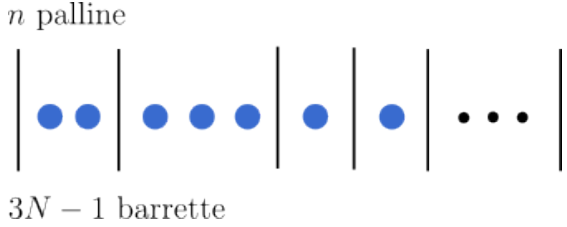
\includegraphics[width=0.5\linewidth]{Immagini/solido di Einstein (microcanonico).png}
    \caption{schema del problema combinatoriale per il solido di Einstein.}
    \label{fig: solido di Einstein (microcanonico)}
\end{figure}
Conoscendo $\Omega(E,N)$ si può determinare l'entropia con la definizione \eqref{eq: entropia (microcanonico)}
\begin{equation}
    S(E,N) = k\log{\frac{(n + 3N -1)!}{n!(3N - 1)!}},
\end{equation}
che nel limite termodinamico, usando l'approssimazione di Stirling \eqref{eq: approssimazione stirling} essendo $E$ ed $N$ molto grandi, diventa
\begin{equation}
    \begin{split}
        S(E,N) &\simeq k[(n + 3N)\log{(n + 3N)} - \cancel{(n + 3N)}  \\
        &- n\log{n} +\cancel{n} - 3N\log{3N} + \cancel{3N}] \\
        &= k[(n + 3N)\log{(n + 3N)} - n\log{n} - 3N\log{3N}]
    \end{split}
\end{equation}
Conoscendo adesso l'entropia si può ricavare la temperatura
\begin{equation}
\label{eq: entropia solido di Einstein (microcanonico)}
    \begin{split}
        \frac{1}{T} = \frac{\p S}{\p E}\bigg|_{N} = \frac{\p n}{\p E}\frac{\p S}{\p n}\bigg|_{N} = \frac{k}{\hbar\omega}[\log{(n + 3N)} - \log{n}] = \frac{k}{\hbar\omega}\log{\frac{n + 3N}{n}},
    \end{split}
\end{equation}
introducendo poi la quantità $\beta := 1/kT$ può essere riscritta come
\begin{equation}
    \beta\hbar\omega = \log{\frac{n + 3N}{n}},
\end{equation}
da cui si ricava la relazione tra il quanto di energia e l'energia del sistema
\begin{equation}
    n = \frac{3N}{e^{\beta\hbar\omega} - 1}.
\end{equation}
L'energia del sistema può quindi essere scritta in funzione di $\beta$, ossia della temperatura $T$, come
\begin{equation}
\label{eq: energia solido di Einstein (microcanonico)}
    E(T,N) = 3N\hbar\omega\bigg(\frac{1}{e^{\beta\hbar\omega} - 1} + \frac{1}{2}\bigg).
\end{equation}
Senza il quanto di energia, non si avrebbe avuto alcunché con cui confrontare $kT$ e quindi non si sarebbe potuto distinguere i limiti di alta e bassa temperatura. Questo è proprio il motivo per cui il problema non può essere affrontato classicamente. I due limiti in questione sono:
\begin{enumerate}
    \item ad alta temperatura, ossia per $kT \gg \hbar\omega$, la granulosità quantistica dell'energia è trascurabile ed, espandendo la \eqref{eq: energia solido di Einstein (microcanonico)}, si ha
    \begin{equation}
    \label{eq: energia solido di Einstein (alta T)}
        E(T,N) \simeq 3N\hbar\omega\bigg(\frac{1}{1 + \beta\hbar\omega + \dots - 1} + \frac{1}{2}\bigg) \simeq 3NkT,
    \end{equation}
    che coincide con il risultato classico, a meno del fattore additivo $1/2$, che non dipende da $\omega$;
    \item a bassa temperatura, ossia per $kT \ll \hbar\omega$, il comportamento del sistema è profondamente quantistico e la \eqref{eq: energia solido di Einstein (microcanonico)} si riduce a 
    \begin{equation}
    \label{eq: energia solido di Einstein (bassa T)}
        E(T,N) \simeq \frac{3N}{2}\hbar\omega + 3N\hbar\omega e^{-\beta\hbar\omega} + \cdots,
    \end{equation}
    dove il primo termine, ovvero l'energia di punto zero, è dominante, quindi tutti gli oscillatori in pratica sono nel loro stato fondamentale di energia $\hbar\omega/2$.
\end{enumerate}
La capacità termica ad $N$ fissato si ottiene da
\begin{equation}
    c_N = \frac{\p E}{\p T}\bigg|_N = \frac{\p \beta}{\p T}\frac{\p E}{\p \beta}\bigg|_N = 3Nk(\beta\hbar\omega)^2\frac{e^{\beta\hbar\omega}}{(e^{\hbar\beta\omega} - 1)^2},
\end{equation}
il cui andamento in funzione di $\beta$ è riportato nel grafico in figura \ref{fig: andamento cap. termica (solido di Einstein)}.
\begin{figure}[h]
    \centering
    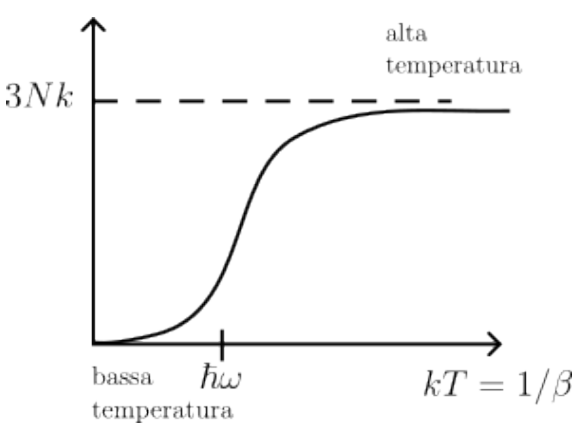
\includegraphics[width=0.4\linewidth]{Immagini/andamento cap. termica (solido di Einstein).png}
    \caption{andamento di $c_N$ in funzione di $\beta$ per il modello di Einstein.}
    \label{fig: andamento cap. termica (solido di Einstein)}
\end{figure}
Il comportamento classico ad alta temperatura si ritrova direttamente dalla \eqref{eq: energia solido di Einstein (alta T)}
\begin{equation}
    c_N \simeq 3Nk,\quad kT \gg \hbar\omega,
\end{equation}
mentre quello a bassa temperatura si ritrova dalla \eqref{eq: energia solido di Einstein (bassa T)} tenendo il primo termine esponenzialmente soppresso, dato che il termine dominante è indipendente da $T$
\begin{equation}
    \begin{split}
        c_N &= \frac{\p\beta}{\p T}\frac{\p}{\p\beta}\bigg(\frac{3N\hbar\omega}{2} + 3N\hbar\omega e^{-\beta\omega\hbar} + \cdots \bigg) \\
        &\simeq 3Nk(\beta\omega\hbar)^2e^{-\beta\omega\hbar},\quad kT \ll \hbar\omega.
    \end{split}
\end{equation}
Tuttavia, l'andamento di $c_N$ per $T \to 0$ non è in accordo con le osservazioni sperimentali, infatti la capacità termica dei solidi reali tende per $T \to 0$ tende a seguire leggi polinomiali; comunque, il modello di Einstein è sicuramente più accurato di quanto possa fare il modello classico, dove $c_N$ è indipendente dalla temperatura.

\subsection{Temperature negative}
Si consideri un sistema quantistico di $N$ componenti distinguibili e interagenti, in cui ognuno di essi abbia a disposizione solo due stati di energia $0$ ed $\epsilon$, come in figura \ref{fig: sistema a due livelli (T negative)}.
\begin{figure}[h]
    \centering
    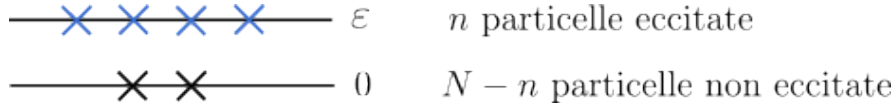
\includegraphics[width=0.7\linewidth]{Immagini/sistema a due livelli (T negative).png}
    \caption{esempio di sistema quantistico non interagente a due livelli.}
    \label{fig: sistema a due livelli (T negative)}
\end{figure}
Un generico microstato di energia $E$ è caratterizzato dal numero $n$ di componenti nel livello $\epsilon$, con gli altri $N - n$ nel livello $0$. L'energia totale del microstato allora è $E = n\epsilon$, da cui si osserva che $n$ determina direttamente $E$. Il numero di microstati $\Omega(E,N)$ con $E$ fissata corrisponde dato dal numero di modi di scegliere $n$ elementi tra le $N$ componenti a disposizione, per cui
\begin{equation}
    \Omega(E,N) = \frac{N!}{n!(N - n)!} =
    \begin{pmatrix}
        N \\
        n
    \end{pmatrix}.
\end{equation}
L'andamento di $\Omega(E,N)$ in funzione di $E$ segue una sorta di gaussiana con picco in $N/2$, come si vede in figura \ref{fig: andamento Omega e S (T negative)}; quindi, da un certo punto in poi $\Omega(E,N)$ decresce all'aumentare di $E$, a differenza di quasi tutti i sistemi.

Le conseguenze di questo comportamento si possono osservare calcolando l'entropia con la definizione \eqref{eq: entropia (microcanonico)} ottenendo
\begin{equation}
    S(E,N) = k\log{\frac{N!}{n!(N - n)!}},
\end{equation}
che nel limite termodinamico, usando l'approssimazione di Stirling dato che $E$ cresce con $N$ insieme a $n$, diventa
\begin{equation}
    S(E,N) = k[N\log{N} - n\log{n} - (N - n)\log{(N - n)}],
\end{equation}
il cui andamento in funzione di $E$ è mostrato in figura \ref{fig: andamento Omega e S (T negative)}. 
\begin{figure}[h]
    \centering
    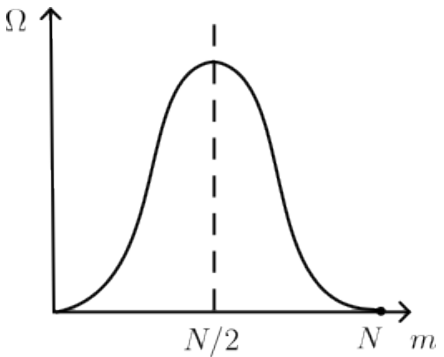
\includegraphics[width=0.36\linewidth]{Immagini/andamento di Omega (T negative).png}
    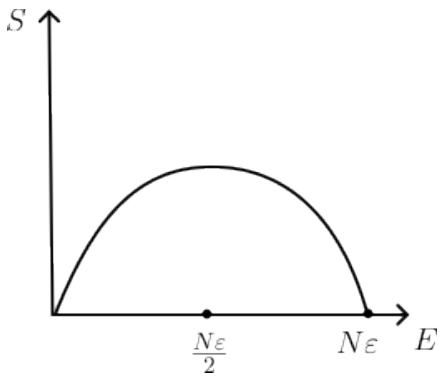
\includegraphics[width=0.35\linewidth]{Immagini/andamento entropia (T negative).png}
    \caption{andamento di: (i) $\Omega(E,N)$ in funzione di $N$; (ii) $S(E,N)$ in funzione dell'energia $E$ di un sistema quantistico non interagente a due livelli.}
    \label{fig: andamento Omega e S (T negative)}
\end{figure}
La particolarità è che $S$ non è una funzione crescente dell'energia, a differenza di quanto assunto normalmente in Termodinamica. A causa di ciò, deve necessariamente esistere una regione dove la temperatura è negativa. Questo accade perché all'aumentare dell'energia, il numero di stati a disposizione diminuisce; ad esempio, nello stato di massima energia esiste un solo modo per ordinare il sistema: tutte le particelle sono nello stato $\epsilon$. Per vedere questa anomalia, si usa l'equazione di stato termica \eqref{eq: equazioni di stato da S} da cui
\begin{equation}
\label{eq: temperature negative I}
    \frac{1}{T} = \frac{k}{\epsilon}\log{\frac{N - n}{n}} \quad\Rightarrow\quad \beta = \frac{1}{\epsilon}\log{\frac{N\epsilon - E}{E}},
\end{equation}
espressione che risulta diventare negativa per valori di energia $E > N\epsilon/2$. Osservando il grafico della funzione inversa, \ref{fig: andamento di beta e T  (T negative)}, si nota che la temperatura cresce fino a $E = N\epsilon/2$, in cui ha una singolarità, per poi cominciare a crescere asintoticamente da $-\infty$. 
\begin{figure}[h]
    \centering
    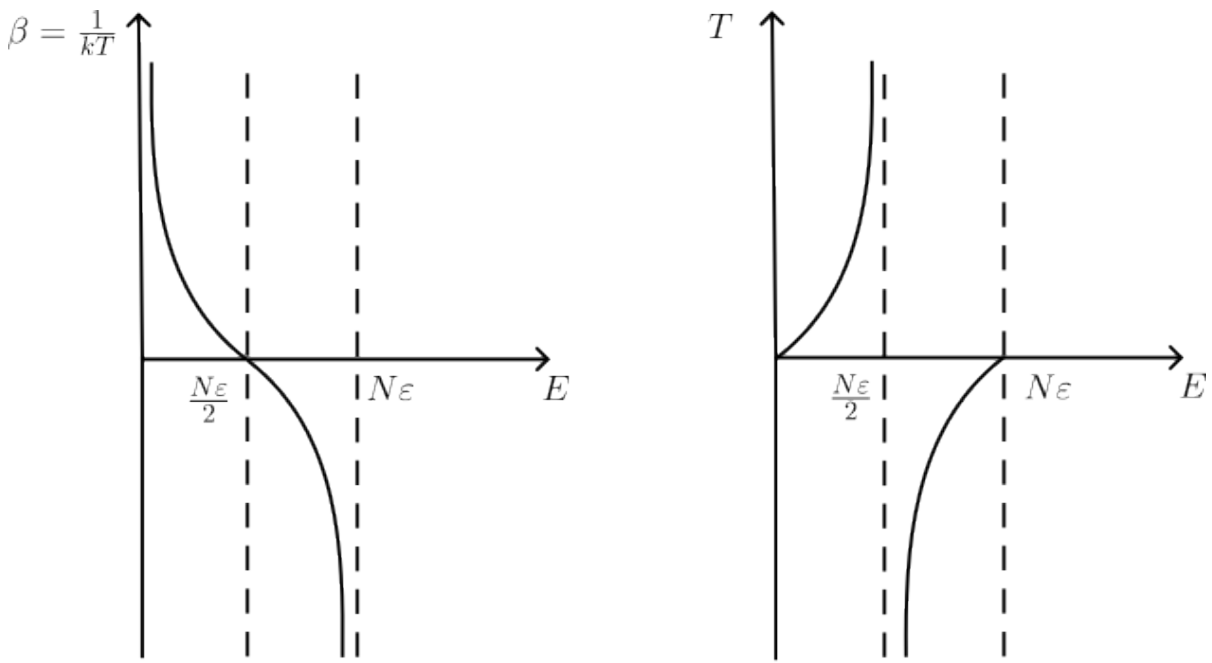
\includegraphics[width=0.7\linewidth]{Immagini/andamento di beta e T (T negative).png}
    \caption{andamento delle funzioni inverse: (i) $\beta(E)$; (ii) $T(E)$.}
    \label{fig: andamento di beta e T (T negative)}
\end{figure}
Quindi, in realtà nella regione in cui $T$ è negativa, la temperatura cresce con l'energia. La relazione \eqref{eq: temperature negative I} può essere invertita per avere
\begin{equation}
    E = \frac{N\epsilon}{1 + e^{\beta\epsilon}} \simeq 
    \begin{cases}
        0,\quad T \to 0^+ \\
        N\epsilon/2,\quad T \to \infty \\
        N\epsilon,\quad T \to 0^-
    \end{cases}
\end{equation}
Ovviamente non è semplice realizzare sperimentalmente dei sistemi che non abbiano altri livelli energetici oltre a $0$ ed $\epsilon$. Questi sistemi non dovrebbero avere nessuna possibilità di vibrare, di spostarsi o altro, altrimenti $\Omega(E)$ continuerebbe a crescere con $E$. Recentemente però sono stati condotti esperimenti con ``cold atoms'' che hanno osservato la presenza di temperature negative, in cui le particelle
si trovano in siti reticolari diversi, permettendo di mantenere la distinguibilità.

\subsection{Eigenvalue Thermalization Hypothesis}
Come detto in precedenza, per un sistema isolato in uno stato puro $\ket{\psi(t)}$, il valore di aspettazione di una generica osservabile $\vmedio{\hatO}_\psi$ non termalizza. L'azione di porsi nell'ensemble microcanonico corrisponde a selezionare gli autostati di energia con autovalori $E_n \in [E, E + \Delta]$, con $\Delta \ll E$. A partire dagli anni '90, si è mostrato che per quasi tutte le hamiltoniane di sistemi non integrabili a molte componenti, ossia per i corrispettivi quantistici dei sistemi ergodici classici, esistono importanti classi di osservabili che in effetti termalizzano. Tuttavia, si tratta solo di variabili locali, cioè definite solo per una sottoregione del sistema globale. Per gli operatori corrispondenti $\hatO$, gli elementi di matrice nella base dell'energia hanno la forma
\begin{equation}
    O_{mn} \simeq \mathcal{A}(E_n)\delta_{nm} + \Omega^{-1/2}\mathcal{A}_2(E_n,E_m)R_{mn},
\end{equation}
dove $\mathcal{A}$ è una funzione ``smoother'' e $R_{mn}$ è una matrice ``random'', estratta da una distribuzione gaussiana, dovuta al fatto che non si possono controllare i comportamenti delle altre particelle del sistema. La probabilità di transire da uno stato all'altro è soppressa dal fattore $\Omega^{-1/2}$. In tal caso, si trova che per quasi tutti i tempi $t$, il valore di aspettazione di $\hatO$ è uguale al valore medio all'equilibrio
\begin{equation}
    \vmedio{\hatO}_\psi = \vmedio{\hatO}_{EQ} \simeq \mathcal{A}(E),
\end{equation}
con una grandezza delle fluttuazioni relative dell'ordine $\Omega^{-1/2}$. Quindi, emerge un comportamento termodinamico per sottosistemi di un sistema quantistico isolato, che può essere espresso in termini della ``entropia di entanglement''. Dato che il sistema globale è in uno stato puro, descritto da $\hatrho(t) = \ket{\psi(t)}\bra{\psi(t)}$, la sua entropia di von Neumann \eqref{eq: definizione entropia von Neumann} è nulla e resta tale durante l'evoluzione del sistema. 

Si supponga ora di dividere i gradi di libertà del sistema in due sottosistemi disgiunti $A$ e $B$. Gli operatori densità relativi $\hatrho_A$ e $\hatrho_B$ si ottengono dalle tracce parziali sui gradi di libertà esterni al sottosistema, ovvero
\begin{equation}
    \hatrho_A = \Tr{\hatrho}_B,\quad \hatrho_B = \Tr{\hatrho}_A.
\end{equation}
Anche se $\hatrho$ corrisponde ad uno stato puro, $\hatrho_A$ e $\hatrho_B$ si riferiscono a stati misti nei due sottosistemi. Si può dimostrare che vale la disuguaglianza 
\begin{equation}
    |\SvN[\hatrho_A] - \SvN[\hatrho_B]| \le \SvN[\hatrho] \le \SvN[\hatrho_A] + \SvN[\hatrho_B],
\end{equation}
da cui, usando il fatto che $\SvN[\hatrho] = 0$ per uno stato puro, si ha
\begin{equation}
    \SvN[\hatrho_A] = \SvN[\hatrho_B] \ge 0.
\end{equation}
Le entropie parziali, o di entanglement, possono quindi crescere durante l'evoluzione del sistema fino a raggiungere il valore di equilibrio $\SvN[\hatrho_{AB}]$ dato da
\begin{equation}
    \SvN[\hatrho_{AB}] \equiv \SvN[\hatrho_A] = \SvN[\hatrho_B].
\end{equation}
La possibilità che le entropie dei due sottosistemi crescano, pur rimanendo nulla l'entropia del sistema globale, appare paradossale.  L'informazione quantistica iniziale, quindi la conoscenza esatta dello stato, non è sparita, ma è accessibile solo tramite misure ``globali'' che non termalizzano. In pratica, il sistema nel suo complesso gioca il ruolo di bagno termico per i sottosistemi.
